%% LyX 2.3.0 created this file.  For more info, see http://www.lyx.org/.
%% Do not edit unless you really know what you are doing.
\documentclass[12pt,english]{article}
\usepackage[T1]{fontenc}
\usepackage[latin9]{inputenc}
\usepackage{geometry}
\geometry{verbose,tmargin=2cm,bmargin=2cm,lmargin=2cm,rmargin=2cm}
\usepackage{xcolor}
\usepackage{float}
\usepackage{booktabs}
\usepackage{textcomp}
\usepackage{url}
\usepackage{amsmath}
\usepackage{graphicx}
\usepackage{setspace}
\usepackage[authoryear]{natbib}
\PassOptionsToPackage{normalem}{ulem}
\usepackage{ulem}
\doublespacing

\makeatletter

%%%%%%%%%%%%%%%%%%%%%%%%%%%%%% LyX specific LaTeX commands.
%% Because html converters don't know tabularnewline
\providecommand{\tabularnewline}{\\}
\providecolor{lyxadded}{rgb}{0,0,1}
\providecolor{lyxdeleted}{rgb}{1,0,0}
%% Change tracking with ulem
\DeclareRobustCommand{\lyxadded}[3]{{\color{lyxadded}{}#3}}
\DeclareRobustCommand{\lyxdeleted}[3]{{\color{lyxdeleted}\lyxsout{#3}}}
\DeclareRobustCommand{\lyxsout}[1]{\ifx\\#1\else\sout{#1}\fi}

%%%%%%%%%%%%%%%%%%%%%%%%%%%%%% Textclass specific LaTeX commands.
\newcommand{\lyxaddress}[1]{
	\par {\raggedright #1
	\vspace{1.4em}
	\noindent\par}
}

%%%%%%%%%%%%%%%%%%%%%%%%%%%%%% User specified LaTeX commands.
\usepackage{ae,aecompl}

\usepackage{lineno} 


\usepackage{xr}
\externaldocument{SupplementaryMaterial}

\makeatother

\usepackage{babel}
\begin{document}

\title{Stabilizing niche differences are required to maintain species-rich
communities in temporally variable environments}

\date{\today}

\author{Coralie Picoche \textsuperscript{{\large{}1,{*}}}, Fr�d�ric Barraquand
\textsuperscript{{\large{}1,2}}}

\maketitle
{\large{}}\textsuperscript{{\large{}1}}{\large{}~University of
Bordeaux, Integrative and Theoretical Ecology, LabEx COTE B�t. B2
- All�e Geoffroy St-Hilaire, 33615 Pessac, France \bigskip{}
}{\large\par}

{\large{}}\textsuperscript{{\large{}2}}{\large{}~CNRS, Institute
of Mathematics of Bordeaux 351 Cours de la Lib�ration, 33405 Talence,
France}{\large\par}

{\large{}\bigskip{}
}{\large\par}

{\large{}\bigskip{}
}{\large\par}

{\large{}\bigskip{}
}{\large\par}

{\large{}\bigskip{}
}{\large\par}

{*} Corresponding author. Email: coralie.picoche@u-bordeaux.fr

\lyxaddress{\pagebreak}

\linenumbers
\begin{abstract}
Explaining coexistence in species-rich communities of primary producers
remains a challenge for ecologists because of the likely competition
for shared resources. Following Hutchinson\textquoteright s seminal
suggestion, many theoreticians have tried to create diversity through
a fluctuating environment, which impairs or slows down competitive
exclusion. There are now several fluctuating-environment models allowing
coexistence, but they often produce only a dozen of coexisting species
at best. Here, we investigate how to create even richer communities
in fluctuating environments, using an empirically parameterized model.
Building on the forced Lotka-Volterra model of Scranton and Vasseur
(2016) inspired by phytoplankton communities, we have investigated
the effect of two coexistence mechanisms, namely the storage effect
and stabilizing niche differences (SNDs). SNDs occur when intraspecific
competition is stronger than interspecific; we tuned the competition
ratio based on empirical data. Although SNDs maintained more species
(50\%) than the storage effect (25\%), we show that none of the two
coexistence mechanisms considered could, by itself, ensure the coexistence
of all species present at the beginning of our simulations. Realistic
seasonal environments only aggravated that picture, as they decreased
persistence relative to white noise. Our results suggest that combining
different mechanisms for biodiversity maintenance into community models
might be more fruitful than trying to find which mechanism explains
best the observed diversity levels. Our results on community composition
(formation of clumps, biomass distribution) in the different scenarios
give further hints about likely coexistence mechanisms at work. 

\textbf{Number of words: 240}
\end{abstract}
\textbf{Keywords: }coexistence; seasonality; competition; phytoplankton;
Lotka-Volterra; storage effect\textbf{}\\

\pagebreak{}

\section{Introduction}

There has been a rich debate in theoretical ecology on how to reconcile
niche and neutral perspectives on species coexistence \citep{gravel_reconciling_2006,carmel_using_2017}.
Under the neutral perspective, all species have equal birth and death
rates and compete equally (since space is limited) whilst under the
niche perspective, birth and death rates can vary between species
and various mechanisms contribute to increasing intraspecific over
interspecific competition \citep{hubbell_unified_2001}. However,
as it has been pointed out repeatedly, niche and neutral processes
are not mutually exclusive: they may actually act together to produce
observed species coexistence \citep{gravel_reconciling_2006,mutshinda_what_2009,gotzenberger_ecological_2012}. 

For instance, \citet{scheffer_self-organized_2006} put forward the
concept of `clumpy coexistence', whereby a simultaneous influence
of both niche and neutral processes create several clumps of similar
species along a single trait axis. Classical stabilizing niche differences
(SNDs) enable coexistence of multiple clumps through stronger net
intraspecific competition \citep{chesson_mechanisms_2000}, while
within-clump coexistence occurs through neutral processes \citep{hubbell_unified_2001,munoz_neutral_2016},
as species that differ too little in their fitnesses cannot exclude
themselves out on reasonable timeframes. Indeed, clumps on the trait
axis eventually thin out in absence of immigration, but transient
coexistence can last for extended periods of time. This `emergent
neutrality' within groups \citep{holt_emergent_2006} has been proposed
as a unifying concept for the niche and neutral theories. The findings
of \citet{scheffer_self-organized_2006} have been disputed due to
hidden niches in the original model \citep{barabas_emergent_2013}.
Hidden niches emerge through stronger intraspecific competition mediated
by a an additional intraspecific predation-like term \citep{barabas_emergent_2013}.
This makes coexistence in the Scheffer and van Nes model more similar
to that of the classical Lotka-Volterra model \citep{barabas_effect_2016},
so that coexistence within clumps is not exactly neutral. Still, the
idea that niche and neutral assembly can mould communities stays potent
\citep{vergnon_interpretation_2013}. Since then, several studies
have suggested that `clumpy coexistence' can occur in theoretical
models, most notably models incorporating temporal variation \citep{scranton_coexistence_2016,sakavara_lumpy_2018}.
In these temporal-variation models, equal competitive strengths are
combined with other mechanisms like the storage effect (or temporal
niche partitioning, that is an equivalent concept for forced Lotka-Volterra
models, \citealp{barabas_community_2012,scranton_coexistence_2016}).
The storage effect increases the possibility of coexistence by making
the interaction strength covary positively with a fluctuating environment
(see also \citealp{barabas_community_2012}). 

Here, we build on the work of \citet{scranton_coexistence_2016} to
investigate the possibility of coexistence through species response
to fluctuating environments. Our enthusiasm for the \citet{scranton_coexistence_2016}
model stems from our interest in phytoplankton communities, that inspired
their thermal preference curves modeling intrinsic growth rates. However,
\citet{scranton_coexistence_2016} described temperature as a white
noise, i.e., independent and identically distributed Gaussian random
variates over time. This appeared to us a key assumption to relax.
Under most latitudes, temperature is indeed a seasonal signal, and
seasonal forcing can strongly affect the dynamics of the community
considered \citep{vesipa_impact_2017}. Hence, over short timescales,
random temporal variations often only add noise to a largely deterministic
seasonal trend. Our present work can therefore be seen as an attempt
to blend \citet{scranton_coexistence_2016}'s framework with the periodic
environments of \citet{barabas_community_2012}, to better represent
the mixture of stochastic and deterministic environmental forces affecting
phytoplankton community dynamics. 

Because many phytoplankton species or genera respond in similar ways
to temperature despite having different optimas \citep{moisan_modelling_2002},
we hypothesized that a large seasonal variation might not necessarily
foster species coexistence. In fact, similar responses to seasonal
fluctuations should lead to an increased synchrony of species abundances
which, in turn, should theoretically mitigate the expected temporal
partitioning. How seasonality affects coexistence (as opposed to a
purely randomly fluctuating environment) is therefore a key feature
of this paper. In particular, we contrast cases where the storage
effect is present vs. absent, which conveniently maps to two different
parameterizations of the forced Lotka-Volterra model. Moreover, the
overall diversity obtained at the end of the simulations with \citet{scranton_coexistence_2016}'s
model was relatively low compared to what we usually observe in phytoplankton
communities (several dozens to hundreds of species). We have therefore
sought out which mechanisms would foster a truly species-rich community
for extended periods of time. 

In an empirical study combining phytoplankton community-level time
series and multivariate autoregressive models \citep{barraquand2018coastal}\footnote{Preprint version available: see \citet{barraquand_weak_2017} in the
reference list}, we found that despite a large influence of the environment (including
temperature, irradiance, and other factors), intraspecific (or intragenus)
competition was most likely the key driver of species coexistence.
In other words, stabilizing niche differences had a large role to
play in maintaining species diversity in coastal phytoplankton \citep{barraquand2018coastal}.
These SNDs mirror those found in a number of terrestrial plant communities
\citep{adler_competition_2018} and in animal communities \citep{mutshinda_what_2009}.

Here, we therefore try to establish what are the relative contributions
of the storage effect vs SNDs to coexistence in a phytoplankton-like
theoretical community model. This led us to cross different combinations
of seasonality in the forcing signal, presence of the storage effect
or not, and intra- vs interspecific competition, in order to disentangle
the contributions of all these factors to biodiversity maintenance.

\section{Methods}

\subsection*{\emph{Models description}}

The model described in \citet{scranton_coexistence_2016} is based
on a variant of the Lotka-Volterra competition model. Fluctuations
in the environment are introduced in the model by temperature-dependent
intrinsic growth rates (see Eq. \ref{eq:modelLV}-\ref{eq:growth},
all coefficients are defined in Table \ref{tab:Coefficients-}) so
that species growth rates can be expressed as:

\begin{eqnarray}
\frac{dN_{i}}{dt} & = & r_{i}(\tau)N_{i}\left(1-\sum_{j=1}^{S}\alpha_{ij}N_{j}\right)-mN_{i}\label{eq:modelLV}\\
r_{i}(\tau) & = & a_{r}(\tau_{0})e^{E_{r}\frac{(\tau-\tau_{\text{0}})}{k\tau\tau_{0}}}f_{i}(\tau)\label{eq:growth}\\
\textnormal{where} & f_{i}(\tau)= & \begin{cases}
e^{-|\tau-\tau_{i}^{opt}|^{3}/b_{i}}, & \tau\leq\tau_{i}^{opt}\\
e^{-5|\tau-\tau_{i}^{opt}|^{3}/b_{i}}, & \tau>\tau_{i}^{opt}
\end{cases}\label{eq:eppley_curve}\\
\textnormal{and} & b_{i}\text{ defined by numerically solving} & \int r_{i}(\tau)d\tau=A\label{eq:niche_breadth}
\end{eqnarray}

Model parameters are detailed in Table \ref{tab:Coefficients-}, and
we set their values to match the features of phytoplankton communities
as in Scranton and Vasseur's work \citeyearpar{scranton_coexistence_2016}.
The niche of each species is defined by its thermal optimum $\tau_{i}^{opt}$.
Thermal performance curves defined in Eq. \ref{eq:eppley_curve} are
parameterized so that all species share the same niche area (Eq. \ref{eq:niche_breadth}),
which sets a trade-off between maximum growth rates and niche width. 

\begin{table}[H]
\caption{Parameter definition and values of the model described in Eq. \ref{eq:modelLV}-\ref{eq:niche_breadth}
\label{tab:Coefficients-}}

\centering{}%
\begin{tabular}{ccc}
\toprule 
Name & Definition & Value (unit)\tabularnewline
\midrule
$S$ & Number of species & 60\tabularnewline
$N_{i}$ & Biomass density of the $i$th species & (kg/area)\tabularnewline
$\tau$  & Temperature & K\tabularnewline
$r_{i}(\tau)$ & Growth rate of species $i$ as a function of temperature & $\frac{\text{kg}}{\text{kg*year}}$\tabularnewline
$\alpha_{ij}$ & Strength of competition of species $j$ on species $i$ & 0.001 area/kg\tabularnewline
$b_{i}$ & Normalization of the thermal decay rate & \tabularnewline
$m$ & Mortality rate & $15\frac{\text{kg}}{\text{kg*year}}$\tabularnewline
$\tau_{0}$ & Reference temperature & 293 K\tabularnewline
$a_{r}(\tau_{0})$ & Growth rate at reference temperature & $386\frac{\text{kg}}{\text{kg*year}}$\tabularnewline
$E_{r}$ & Activation energy & 0.467 eV\tabularnewline
$k$ & Boltzmann's constant & $8.6173324.10^{-5}\text{eV.K}^{-1}$\tabularnewline
$f_{i}(\tau)$ & Fraction of the maximum rate achieved for the $i$th species & \tabularnewline
$\mu_{\tau}$ & Mean temperature & 293 K\tabularnewline
$\sigma_{\tau}$ & Standard deviation for temperature & 5 K\tabularnewline
$\tau_{\text{min}}$ & Minimum thermal optimum & 288K\tabularnewline
$\tau_{\text{max}}$ & Maximum thermal optimum & 298 K\tabularnewline
A & Niche breadth & $10^{3.1}\frac{\text{kg}}{\text{kg*year}}$ \tabularnewline
$\tau_{i}^{\text{opt}}$ & Thermal optimum for growth of the $i$th species & K\tabularnewline
$\theta$ & Scaling between white noise and seasonal signal & {[}0,$\sqrt{(}2)${]}\tabularnewline
$\rho$ & Ratio of intra-to-intergroup competition strengths & (1;10)\tabularnewline
\bottomrule
\end{tabular}
\end{table}

We kept the mean and standard deviation of the forcing signal but
included a lower-frequency component using a sinusoidal function with
a period of 365 days (1 time unit being one day, Eq. \ref{eq:Seasonal_signal}).
We tune the ratio of low-to-high frequency with the variable $\theta$
so as to keep the same energy content - i.e., equal total variance
- in the forcing signal.

\begin{equation}
\tau(t)=\mu_{\tau}+\theta\sigma_{\tau}\sin\left(\frac{2\pi t}{365}\right)+\epsilon_{t},\text{where }\epsilon_{t}\sim\mathcal{N}(0,\sigma_{\tau}\sqrt{1-\frac{\theta^{2}}{2}})\label{eq:Seasonal_signal}
\end{equation}

Note that the upper limit for $\theta$, $\sqrt{2}$, corresponds
to a completely deterministic model which we do not explore here (but
see \citet{zhao1991qualitative} proving bounded coexistence). We
chose to keep the stochasticity in the signal and to model a plausible
temperature signal with $\theta=1.3$ (see Fig. \ref{fig:Times-series_temperature_species}b)
when considering a seasonal forcing of the dynamics.

The formulation of the forced Lotka-Volterra model of \citet{scranton_coexistence_2016}
implies a storage effect, as the competition strengths covary positively
with the growth rate values $r_{i}(\tau)$\citep{chesson_multispecies_1994,ellner_how_2016}.
To test for the effect of an explicit storage effect in the model,
we formulated a new version of this model, where we removed this assumption
by using the mean value of a species' growth rate ($\bar{r_{i}}$)
to weight the interaction coefficients (see Table \ref{tab:ModelsOfGrowthRates}).

\begin{equation}
\frac{dN_{i}}{dt}=N_{i}\left(r_{i}(\tau)-\sum_{j=1}^{S}\bar{r}_{i}\alpha_{ij}N_{j}\right)-mN_{i}\label{eq:eqLV_noforcecompetition}
\end{equation}

In this way, competition strengths remain unaffected by the environmental
conditions, in contrast to growth rates (Eq. \ref{eq:eqLV_noforcecompetition}),
while preserving the same average magnitude as in Eq. \ref{eq:modelLV}.

Stabilizing niche differences are ensured by the addition of the coefficient
$\rho$, which is the ratio of intra-to-intergroup competition strength.
We can therefore re-write the interaction coefficients $\alpha_{ij}$
in Eq. \ref{eq:alpha_def}

\begin{equation}
\alpha_{ij}=\alpha\left(1+(\rho-1)\delta_{ij}\right)\label{eq:alpha_def}
\end{equation}

where $\delta_{ij}$ is the Kronecker symbol, equal to 1 if $i=j$
and to 0 otherwise. The value of the parameter $\rho=10$ was chosen
from analyses of phytoplanktonic data \citep{barraquand2018coastal}
\footnote{The values of non-zero interspecific competition coefficients reported
in Fig. 5 of \citet{barraquand2018coastal} are somewhat higher than
here (and $\rho$ lower, closer to 4) because the best-fitting model
actually set to zero some intergroup competition coefficients; using
a model where all $\alpha_{ij}$ are non-zero leads in contrast to
$\rho=10$. }. 

In addition to two types of environmental forcings (white noise with
$\theta=0$, and seasonal forcing with $\theta=1.3$), we therefore
compare the results for four formulations of the model: with and without
an explicit storage effect (Eq. \ref{eq:modelLV} and Eq. \ref{eq:eqLV_noforcecompetition},
respectively) ; with and without stabilizing niche differences ($\rho=10$
or $\rho=1$, respectively). These are summed up in Table \ref{tab:ModelsOfGrowthRates}
\begin{center}
\begin{table}[H]
\begin{centering}
\begin{tabular}{ccc}
\hline 
$\frac{dN_{i}}{dt}+mN_{i}$ & Storage effect & No storage effect\tabularnewline
\hline 
Stabilizing niche differences & $r_{i}(\tau)N_{i}\left(1-\sum_{j=1}^{S}\alpha\left(1+9\delta_{ij}\right)N_{j}\right)$ & $N_{i}\left(r_{i}(\tau)-\sum_{j=1}^{S}\bar{r}_{i}\alpha\left(1+9\delta_{ij}\right)N_{j}\right)$\tabularnewline
\hline 
No stabilizing niche differences & $r_{i}(\tau)N_{i}\left(1-\sum_{j=1}^{S}\alpha N_{j}\right)$ & $N_{i}\left(r_{i}(\tau)-\sum_{j=1}^{S}\bar{r}_{i}\alpha N_{j}\right)$\tabularnewline
\hline 
\end{tabular}
\par\end{centering}
\caption{\label{tab:ModelsOfGrowthRates}Growth rate of species $i$ in the
four formulations of the model we present}
\end{table}
\par\end{center}

\subsection*{Set-up}

We replicate the `Species sorting' experiment of \citet{scranton_coexistence_2016}
so as to investigate how the structure of synthetic phytoplankton
communities varies under the different scenarios we described above.
We focused on the dynamics of a community initialized with 60 species
with thermal optima uniformly spaced along the interval {[}15�C, 25�C{]},
and with the same initial density $\left(\frac{\ensuremath{1}}{\alpha S}\right)$.
Each simulation was run for 5000 years in 1-day intervals. When the
density of a species dropped below $10^{-6}$, it was considered extinct.
For each combination of parameters (type of environmental signal,
storage effect and stabilizing niche differences), we ran 100 simulations. 

All simulations were ran with Matlab's ode45 algorithm, an explicit
Runge-Kutta (4,5) algorithm with an absolute error tolerance of $10^{-8}$,
and relative error tolerance $10^{-3}$. The code is available in
a GitHub repository \footnote{\url{https://github.com/CoraliePicoche/Seasonality}, will be made
public upon acceptance or at the reviewer's request} .

\section{Results }

Typical dynamics of the community following Eq. \ref{eq:modelLV}
(the model of \citealp{scranton_coexistence_2016}), with both the
environmental signals described in Eq. \ref{eq:modelLV} (original
choice of \citealp{scranton_coexistence_2016}; Fig. \ref{fig:Times-series_temperature_species}a)
and Eq. \ref{eq:Seasonal_signal} (our variant, Fig. \ref{fig:Times-series_temperature_species}b),
are shown in Fig. \ref{fig:Times-series_temperature_species}c and
d. A sinusoidal forcing produces the strongly seasonally structured
dynamics that are typical of phytoplankton. Even though only 5 species
can be seen in Fig. \ref{fig:Times-series_temperature_species}c,
there were 14 species still present at the end of the simulation forced
by a white noise, with large disparities in the range of variation
of their biomasses. A third of the species kept a biomass above 10
kg/area (setting area = 1 ha, with a depth of a few meters, produce
a realistic standing biomasses; \citealp{reynolds2006ecology}) while
6 out of the 14 remained below the unit. All persisting species in
the white noise simulations were clustered within a 3.2�C-range of
thermal optima (see the biomass distribution as a function of the
thermal optimum in Fig. A1 in the Supplementary Material). No obvious
temporal patterns (e.g., cycles) could be seen in the communities
forced by white noise. On the contrary, seasonal cycles were clear
in the seasonally-forced case of Fig. \ref{fig:Times-series_temperature_species}d.
Only 4 species coexisted at the end of the simulation with seasonal
forcing, gathered in two groups with large thermal optimum differences
(5.7�C between the maximum thermal optimum of the first group and
the minimum thermal optimum of the second group). When temperatures
are high, the group with higher thermal optima reaches its maximum
biomass, then as temperature decreases through the season, these species
leave room for the growth of the low-temperature group.

\begin{figure}[H]
\begin{centering}
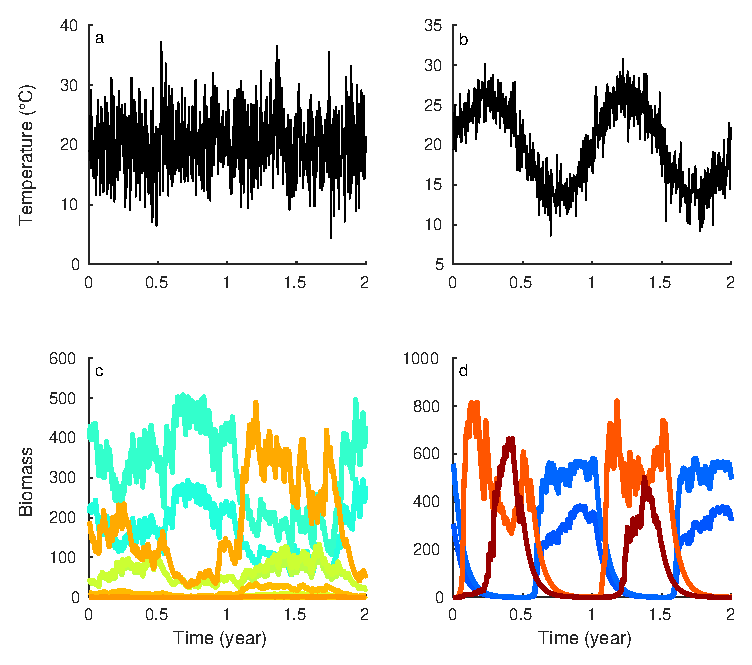
\includegraphics[width=0.95\textwidth]{graphe/Fig1}
\par\end{centering}
\caption{Time series of temperature (top; a-b) and extant species (bottom;
c-d) for the 2 last years of a 5000 years simulation, with storage
effect and no stabilizing niche differences. The forcing temperature
is either a white noise (a) or a noisy seasonal signal (b), leading
to community dynamics with more erratic fluctuations (c) vs seasonally
structured fluctuations (d). Line colors of species biomasses correspond
to their thermal optimum (from blue, corresponding to low thermal
optimum, to red, corresponding to high thermal optimum).\label{fig:Times-series_temperature_species}}
\end{figure}

The decrease in persistence due to seasonality observed in Fig. \ref{fig:Times-series_temperature_species}
was confirmed in all our simulations (Fig. \ref{fig:Persistence-of-species}).
In cases where final species richness varied from one simulation to
another (namely, the two middle cases in Fig. \ref{fig:Persistence-of-species}:
with storage effect but without stabilizing niche differences, or
without storage effect but with stabilizing niche differences), seasonality
reduced the number of extant species to, on average, 27\% and 48\%
of their original values, respectively (Fig. \ref{fig:Persistence-of-species}).
A seasonal signal therefore led to a much smaller average persistence.
There was also less variance in persistence between seasonally forced
simulations when compared to white noise simulations. 

Both the stabilizing niche differences and the storage effect markedly
increased persistence. Without any of these coexistence mechanisms,
only one species persisted at the end of the simulations. When only
the storage effect was present, the number of extant species varied
between 8 and 20 (14.8 $\pm$ 2.4) with a white noise, or 2 and 6
(4.1 $\pm$ 0.7) with a seasonal signal. On the other hand, when only
stabilizing niche differences were present, the number of extant species
nearly doubled, varying between 20 and 32 (27.5 $\pm$ 2.4), or 12
and 15 (13.3 $\pm$ 0.6), with a white noise or a seasonal signal,
respectively. Remarkably, when the storage effect and SNDs both affected
the community dynamics, all species persisted in the community, while
neither of these mechanisms was able to produce that result alone,
for either white noise and seasonal forcing.

\begin{figure}[H]
\begin{centering}
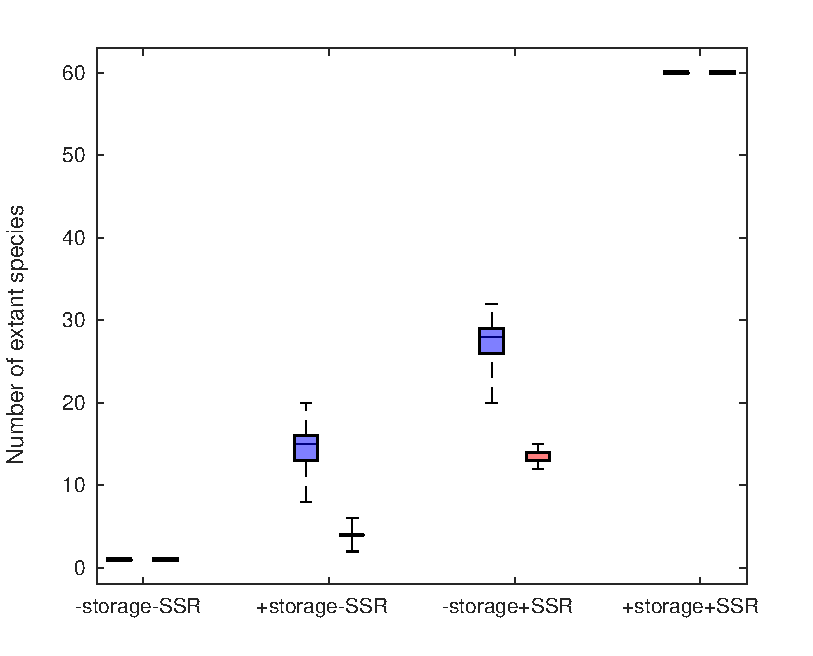
\includegraphics[width=0.75\textwidth]{graphe/Fig2}
\par\end{centering}
\caption{Number of species still present at the end of 100 simulations (5000
years each), initialized with 60 species, with a white noise forcing
signal (blue) or a noisy seasonal signal (red). The signs + or - storage
refer to presence or absence of a storage effect, respectively; +
/ - SND, presence or absence of Stabilizing Niche Differences, respectively.
Community compositions are stable in the cases -storage-SND and +storage+SND,
for which 1 or 60 species are still present at the end of all simulations,
respectively. Due to low variance, the whiskers here represent min
and max rather than 1.5 interquartile range. \label{fig:Persistence-of-species} }
\end{figure}

When the richness of the community was stable (either 1 or 60 species
at the end of the simulation), there were still large differences
in the structure of the community with respect to temperature, due
to both stochasticity and the type of forcing (Fig. \ref{fig:Mean-biomass-in_stable_cases}).
Without storage effect nor SNDs, a white noise forcing favored species
with intermediate thermal optima, with two thirds of the simulations
ending with a species with a thermal optimum between 18.9�C and 21.4�C
(corresponding to only one fourth of the range of thermal optima present
at the beginning of the simulation) and reaching a maximum average
biomass in this range (Fig. \ref{fig:Mean-biomass-in_stable_cases}a).
This distribution can be related to a selection for the highest long-term
growth rates, averaged over time (see scaled growth rates in Fig.
\ref{fig:Mean-biomass-in_stable_cases}). On the contrary, seasonality
tended to favor species with larger maximum growth rates (thermal
optima above 22�C). Species with a higher thermal optimum are more
likely to persist and to reach a higher biomass at the end of the
simulation. 38\% of the simulations therefore ended with the species
having the highest temperature optimum, 25�C. 

When both coexistence mechanisms were present, the 60 initial species
coexisted with small variations in biomasses for each species over
the 100 simulations (mean CV=0.008 across simulations with either
a white noise or a seasonal forcing signal, Fig. \ref{fig:Mean-biomass-in_stable_cases}b
and d). The forcing signal modified only the distribution of biomasses
resulting in contrasted community structures despite equal richness
in both simulation types. With a white noise, the distribution was
unimodal with a maximum biomass reached for the second best long-term
average growth rate (corresponding to a thermal optimum of 20.2�C).
On the contrary, a seasonal signal led to a bi-modal distribution
(centered on 17.0�C and 24.4�C), each corresponding to one season,
with highest biomasses for higher thermal optima (Fig. \ref{fig:Mean-biomass-in_stable_cases}d).
The minimum biomass was reached for the best long-term average growth
rate at an intermediate temperature (20.4�C), one species apart from
the maximum biomass in the white noise case. 

\begin{figure}[H]
\begin{centering}
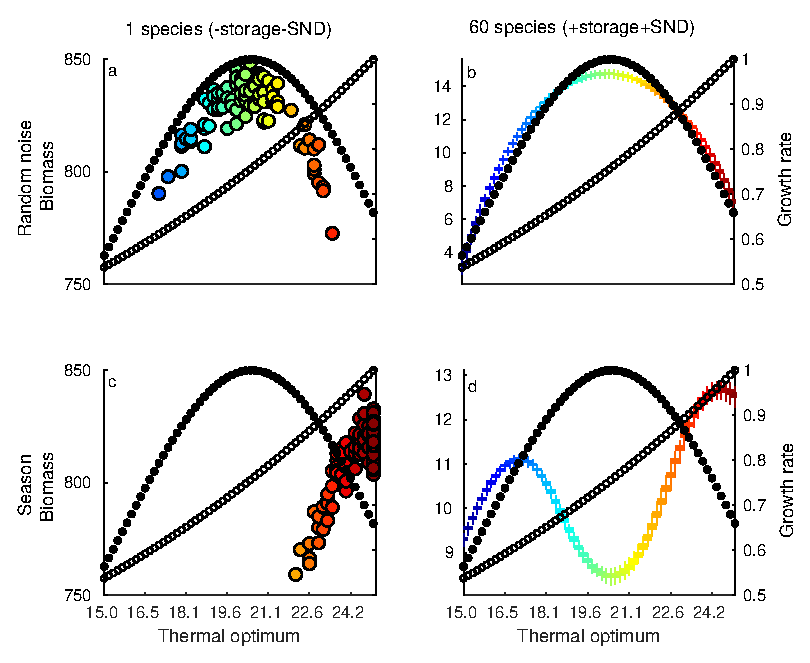
\includegraphics[bb=0bp 0bp 356bp 296bp,width=0.95\textwidth]{graphe/Fig3}
\par\end{centering}
\caption{Mean biomass distribution over the last 200 years for 100 simulations,
as a function of the species thermal optima. Here we consider the
two stable-composition cases and two types of forcing signal. On the
left column, simulations without storage effect nor stabilizing niche
differences are presented. Only one species is present at the end
of the simulations and its mean value is represented by one large
colored circle per simulation. There can be several circles for the
same species, corresponding to multiple simulations ending with this
species alone. On the right column, simulations with storage effect
and stabilizing niche differences are represented. All species are
present at the end of the simulations and small boxplots present the
variation in the temporal average of biomass with a given trait, for
100 simulations. The forcing signal is either a white noise (top)
or a seasonal signal (bottom). Each species is identified by its thermal
optimum through its color code. Scaled (divided by maximum) average
and maximum growth rates are shown as small filled and open circles,
respectively, and are indexed on the right y-axis. \label{fig:Mean-biomass-in_stable_cases}}
\end{figure}

In cases where the richness of the community varied, the overall shape
(multimodal vs. unimodal) of the marginal distribution of extant species
with respect to the trait axis were similar for both types of environmental
forcings (Fig. \ref{fig:Unstable_cases}). By contrast, the type of
coexistence mechanism generated different shapes. Indeed, the storage
effect led to a multimodal biomass distribution with respect to thermal
optima. We always observed 3 modes with a white noise and 3 modes
in 95\% of the seasonal simulations (Fig. \ref{fig:Unstable_cases}a).
With a white noise, extant species are grouped in rather similar clumps
regarding species thermal optima (between 18.8�C and 22.2�C) whereas
clumps tended to be further apart in the seasonal case, covering a
total range of 7.7�C, with species grouping in the higher part of
the thermal range, above 22�C. On the other hand, stabilizing niche
differences led to a quasi-uniform biomass distribution (Fig. \ref{fig:Unstable_cases}
b). Species characterising communities forced by a white noise stayed
in the lower range of temperatures (in 96\% of the simulations, the
highest thermal optimum was 22.4�C, see Fig. A2 in the Supplementary
Material) while they were filtered out in communities subjected to
a seasonal fluctuation of their environment, for which species with
thermal optima above 20.5�C persisted.

\begin{figure}[H]
\begin{centering}
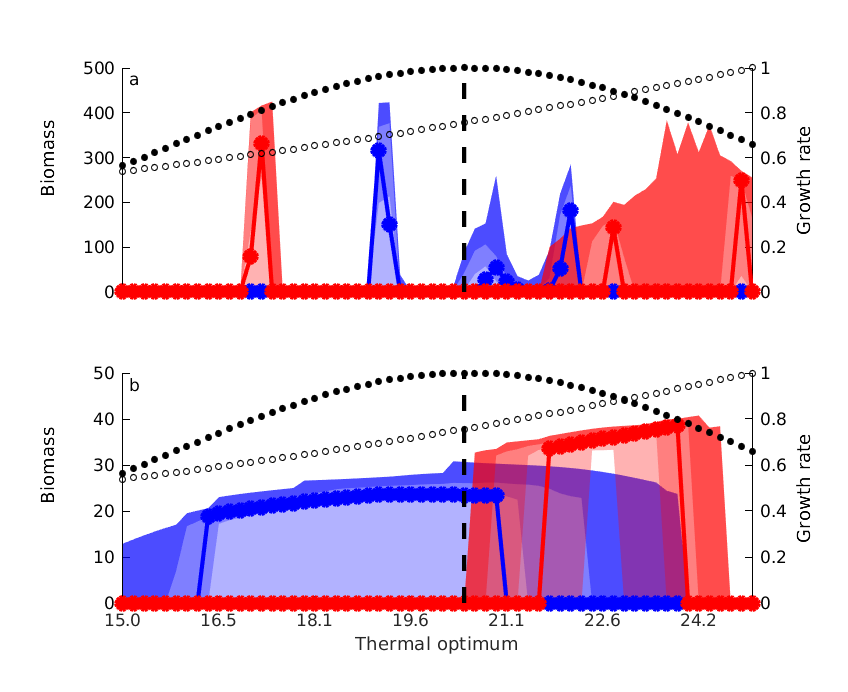
\includegraphics[bb=0bp 0bp 428bp 338bp,width=0.85\textwidth]{graphe/Fig4}
\par\end{centering}
\caption{Mean biomass distribution over the last 200 years for 100 simulations,
as a function of thermal optima, with storage effect and no stabilizing
niche differences (a) and without storage effect, with stabilizing
niche differences (b). The forcing signal is either a white noise
(in blue) or a seasonal signal (in red). Shades of the same color
correspond to the 50th, 90th and 100th percentiles of the distributions
while colored lines correspond to one representative simulation. Scaled
(divided by maximum) average (whose maximum is indicated by the dashed
line) and maximum growth rates are shown as filled and open and circles,
respectively, and indexed on the right y-axis. \label{fig:Unstable_cases}}
\end{figure}


\section{Discussion}

We have simulated competitive Lotka-Volterra dynamics forced by a
fluctuating environment (e.g., temperature fluctuations) under a range
of scenarios allowing more or less coexistence. Two coexistence mechanisms,
the storage effect and stabilizing niches differences, could be either
present or absent, which led to four scenarios. These four scenarios
were crossed with two possibilities for the forcing signal, a white
noise and a stochastic yet seasonal signal, both with equal temporal
variance. Our investigation therefore built on the model of \citet{scranton_coexistence_2016},
which included a white noise forcing and a storage effect, but considered
seven additional combinations of mechanisms. This was motivated by
our wish to include two observed features of phytoplankton dynamics:
seasonal cycles \citep{winder_annual_2010} and stabilizing niche
differences \citep{chesson_mechanisms_2000,adler_coexistence_2010,barraquand2018coastal}.
Stabilizing niche differences, that occur whenever intraspecific competition
is stronger than interspecific competition, can arise from many mechanisms:
nonlinearities in the functional forms of competition or mutualism
that contribute to increasing self-regulation \citep{kawatsu2018density},
predation or parasitism (see e.g., the generalist predators in \citealp{haydon1994pivotal}),
etc. They seem nonetheless an ubiquitous feature in primary producers
\citep{adler_competition_2018}.

We have found that first, temporally forced Lotka-Volterra dynamics
cannot sustain any diversity with our phytoplankton-based set of parameters,
unless the structure is geared to include either a storage effect
or SNDs. Although this absence of diversity-enhancing effect of ``pure''
environmental variation has already been stated by other authors \citep{barabas_community_2012,fox_intermediate_2013,scranton_coexistence_2016},
this is not always intuitive \citep{fox_intermediate_2013}, so we
feel compelled to stress it once more: temporal variation in growth
rate alone cannot help coexistence within competitive communities.
A nice point made by \citet{scranton_coexistence_2016} was that a
built-in storage effect in a forced Lotka-Volterra model, parameterized
for phytoplankton communities, could lead to some degree of coexistence.
Our investigation reproduced these results, using the white noise
forcing considered by \citet{scranton_coexistence_2016}. However,
an arguably more lifelike noisy and seasonal temperature forcing considerably
lessened the richness of the community after 5000 years, decreasing
from 15 to 4 species on average. Even imagining that groups represented
here are genera or classes rather than species, this is a fairly low
diversity for a phytoplankton-like community (see Chapter 1 in \citealp{reynolds2006ecology}).
This suggests that the storage effect may not, on its own, be sufficient
to maintain species-rich communities (e.g., dozens to hundreds of
species). We have therefore sought out whether stabilizing niche differences
could maintain a higher diversity, using field-based intra- vs intergroup
(species or genera) competition strength ratio \citep{barraquand2018coastal},
where the intragroup density-dependence was chosen 10 times stronger.
On their own, SNDs produced a higher level of diversity than the storage
effect (almost double for white noise), which not only aligns with
our results on phytoplankton but also with results on perennial plants
\citep{adler_coexistence_2010}. 

However, the seasonal forcing still considerably reduced diversity
when only SNDs were considered, especially the ``neutral'' kind
of diversity, i.e., diversity within clumps of similar traits. This
diversity reduction occurs because within a season, the signal autocorrelation
gives long, contiguous time intervals to the best competitor to exclude
its less adapted heterospecifics. This makes the results likely to
hold not only for seasonal environments, but more generally for autocorrelated
ones, i.e., ``red'' noise. This could be relevant for species whose
population dynamics occurs at timescales largely above one year. In
contrast, a white noise generates large temperature shifts more frequently,
and thereby forbid such competitive exclusion. In a seasonal setting,
a species with the highest long-term averaged growth rate may not
be the best competitor, and can disappear as a result of a strong
competition from both low- and high-temperature tolerant species.
This holds with or without a storage effect. 

Our results may appear at odds with recent proposals that seasonal
forcing in itself would help maintain diversity \citep{sakavara_lumpy_2018}.
However, we compared the effect of seasonal forcing to that of other
forcing signals while controlling for total variance. Thus, the contrast
between our results and those of \citet{sakavara_lumpy_2018} may
be due to the role of forcing variance over time (we compare scenarios
under a constant total variance). Overall, while seasonality may be
slightly better than no forcing at all in maintaining diversity, seasonal
forcing of parameters does not improve coexistence: diversity within
clumps is lower when seasonality is included.

In addition to community diversity, the biomass-trait relationship
also varied from one simulation to another. Some regularities did
emerge across simulations though. The storage effect begot several
clumps along the trait space (as observed by \citealp{scranton_coexistence_2016}).
The seasonality that we added to the temperature signal led to more
distant clumps on the trait axis (as said above, less species per
clump). Conversely, SNDs alone led to relatively uniform biomass distributions,
with species forming a single large cluster, which covers a fraction
of the initial trait space. The identification of multiple modes in
biomass-trait relationships and SADs is relatively recent \citep{dornelas_multiple_2008,matthews_multimodal_2014}
and is a rare pattern in theoretical models \citep{mcgill_species_2007}.
\citet{barabas_emergent_2013} convincingly argued that multimodality
could arise from the demographic stochasticity of a single model run
(with either SNDs or neutrality, but without the clumpy coexistence
emerging from a storage effect). However, our results are based on
many model runs, for which either the storage effect alone or a storage
effect + SNDs in a seasonal context consistently produced multimodal
distributions, while simulations without the storage effect always
led to a single cluster along the trait axis. Our suggestion for empirical
studies is as follows: if only one spatial location is observed, caution
in interpreting multiple clumps on the trait axis is of course required,
as \citet{barabas_emergent_2013} highlighted. However, with several
locations - or in a theoretical context - one could average across
locations to reproduce similar graphs to the ones produced here. Clumps
in the trait axis when averaged across model runs/locations is therefore
a signature of the storage effect for the cases that we considered
in the article. Of course, other mechanisms that we did not include
in our models may produce similar patterns \citep{rael2018emergent}.
Still, clustering on the trait axis, in scenarios where the environment
fluctuates strongly in time, suggests that storage effects could be
at work.

In our previous empirical study of coastal phytoplankton dynamics
\citep{barraquand2018coastal}, we did not find any storage effect
(which does not mean that it could not be observed in other systems).
Given the results on species richness and composition presented here,
we are skeptical that the storage effect alone could help explaining
phytoplankton diversity. However, our results suggest that in phytoplankton-like
seasonal environments, even though empirically-based SNDs produce
much more diversity than the storage effect when considered in isolation,
the storage effect can help diversity maintenance when combined to
other mechanisms. Indeed, the combination storage effect + SNDs is
non-additive: the cases were both SNDs and the storage effect were
present showed more diversity than generated by any mechanism on its
own. 

The above results suggest the very exciting idea that multiple coexistence
mechanisms might combine superadditively, thus helping us to better
understand the astounding diversity of primary producers. This logic
could, in principle, be extended to mechanisms that we have not considered
here (e.g., spatial structure, specialized natural enemies, that could
be as important here for plankton as they are for tropical trees,
see \citealp{bagchi_pathogens_2014,comita_testing_2014,stump_distance-responsive_2015,barraquand_weak_2017}).
Previous research has however demonstrated that generalist seed predation
could weaken the storage effect \citep{kuang_coexistence_2009,kuang_interacting_2010}
thus different mechanisms might not always combine superadditively
as we found here. That said, superadditivity has been found in some
cases, i.e., pathogens could enhance the storage effect \citep{mordecai_pathogen_2015}.
Better explaining plant or microbial diversity would then not be about
selecting the best unique mechanism susceptible to explain the observed
diversity, but rather better combining those mechanisms together.
This may obviously be an annoyance for those who like to sharpen Occam's
razor, but it clearly holds opportunities for theoreticians wishing
to investigate synergies between coexistence mechanisms in highly
diverse communities. Aside from the synergies between predator diversity-enhancing
effects and SNDs or storage effects (on the temporal axis), one obvious
follow-up of this research would be interactions with spatial structure.
Spatial structure occurs both endogeneously, through spatially restricted
movements and interactions, and exogeneously, through spatial variation
in environmental covariates \citep{bolker_combining_2003}. Numerous
studies \citep[e.g.,][]{bolker_spatial_1999,murrell_2002} have shown
that spatially restricted movements and interactions - very small-scale
spatial structure - can help coexistence, which we believe would be
especially important for phytoplankton since many species form colonies
(\citealp{reynolds2006ecology}; see discussion in \citealp{barraquand2018coastal}).
Moreover, although temperature is usually relatively spatially homogeneous
over space, other drivers (e.g., rainfall, pH in terrestrial ecosystems;
salinity in aquatic ones) may exhibit spatial variation which is a
main factor for coexistence \citep{snyder_when_2008}. The odds that
different (resource) niches, natural enemies, spatial limits to competition
and temporal niche partitioning all interact to promote the very high-dimensional
coexistence observed in the field seem much higher than for any of
those mechanisms alone. Whether the diversity-enhancing effects of
these mechanisms combine sub-additively (as in \citealp{kuang_interacting_2010})
or super-additively like here is therefore worthy of further research. 

\section*{Acknowledgements}

We thank Alix Sauve for numerous thoughtful comments and some bibliographic
references. This study was supported by the French ANR through LabEx
COTE (ANR-10-LABX-45).

\bibliographystyle{../spbasic_nicer}
\bibliography{coexistence}

\end{document}
